\pgfdeclareplotmark{cross} {
\pgfpathmoveto{\pgfpoint{-0.3\pgfplotmarksize}{\pgfplotmarksize}}
\pgfpathlineto{\pgfpoint{+0.3\pgfplotmarksize}{\pgfplotmarksize}}
\pgfpathlineto{\pgfpoint{+0.3\pgfplotmarksize}{0.3\pgfplotmarksize}}
\pgfpathlineto{\pgfpoint{+1\pgfplotmarksize}{0.3\pgfplotmarksize}}
\pgfpathlineto{\pgfpoint{+1\pgfplotmarksize}{-0.3\pgfplotmarksize}}
\pgfpathlineto{\pgfpoint{+0.3\pgfplotmarksize}{-0.3\pgfplotmarksize}}
\pgfpathlineto{\pgfpoint{+0.3\pgfplotmarksize}{-1.\pgfplotmarksize}}
\pgfpathlineto{\pgfpoint{-0.3\pgfplotmarksize}{-1.\pgfplotmarksize}}
\pgfpathlineto{\pgfpoint{-0.3\pgfplotmarksize}{-0.3\pgfplotmarksize}}
\pgfpathlineto{\pgfpoint{-1.\pgfplotmarksize}{-0.3\pgfplotmarksize}}
\pgfpathlineto{\pgfpoint{-1.\pgfplotmarksize}{0.3\pgfplotmarksize}}
\pgfpathlineto{\pgfpoint{-0.3\pgfplotmarksize}{0.3\pgfplotmarksize}}
\pgfpathclose
\pgfusepathqstroke
}
\pgfdeclareplotmark{cross*} {
\pgfpathmoveto{\pgfpoint{-0.3\pgfplotmarksize}{\pgfplotmarksize}}
\pgfpathlineto{\pgfpoint{+0.3\pgfplotmarksize}{\pgfplotmarksize}}
\pgfpathlineto{\pgfpoint{+0.3\pgfplotmarksize}{0.3\pgfplotmarksize}}
\pgfpathlineto{\pgfpoint{+1\pgfplotmarksize}{0.3\pgfplotmarksize}}
\pgfpathlineto{\pgfpoint{+1\pgfplotmarksize}{-0.3\pgfplotmarksize}}
\pgfpathlineto{\pgfpoint{+0.3\pgfplotmarksize}{-0.3\pgfplotmarksize}}
\pgfpathlineto{\pgfpoint{+0.3\pgfplotmarksize}{-1.\pgfplotmarksize}}
\pgfpathlineto{\pgfpoint{-0.3\pgfplotmarksize}{-1.\pgfplotmarksize}}
\pgfpathlineto{\pgfpoint{-0.3\pgfplotmarksize}{-0.3\pgfplotmarksize}}
\pgfpathlineto{\pgfpoint{-1.\pgfplotmarksize}{-0.3\pgfplotmarksize}}
\pgfpathlineto{\pgfpoint{-1.\pgfplotmarksize}{0.3\pgfplotmarksize}}
\pgfpathlineto{\pgfpoint{-0.3\pgfplotmarksize}{0.3\pgfplotmarksize}}
\pgfpathclose
\pgfusepathqfillstroke
}
\pgfdeclareplotmark{newstar} {
\pgfpathmoveto{\pgfqpoint{0pt}{\pgfplotmarksize}}
\pgfpathlineto{\pgfqpointpolar{44}{0.5\pgfplotmarksize}}
\pgfpathlineto{\pgfqpointpolar{18}{\pgfplotmarksize}}
\pgfpathlineto{\pgfqpointpolar{-20}{0.5\pgfplotmarksize}}
\pgfpathlineto{\pgfqpointpolar{-54}{\pgfplotmarksize}}
\pgfpathlineto{\pgfqpointpolar{-90}{0.5\pgfplotmarksize}}
\pgfpathlineto{\pgfqpointpolar{234}{\pgfplotmarksize}}
\pgfpathlineto{\pgfqpointpolar{198}{0.5\pgfplotmarksize}}
\pgfpathlineto{\pgfqpointpolar{162}{\pgfplotmarksize}}
\pgfpathlineto{\pgfqpointpolar{134}{0.5\pgfplotmarksize}}
\pgfpathclose
\pgfusepathqstroke
}
\pgfdeclareplotmark{newstar*} {
\pgfpathmoveto{\pgfqpoint{0pt}{\pgfplotmarksize}}
\pgfpathlineto{\pgfqpointpolar{44}{0.5\pgfplotmarksize}}
\pgfpathlineto{\pgfqpointpolar{18}{\pgfplotmarksize}}
\pgfpathlineto{\pgfqpointpolar{-20}{0.5\pgfplotmarksize}}
\pgfpathlineto{\pgfqpointpolar{-54}{\pgfplotmarksize}}
\pgfpathlineto{\pgfqpointpolar{-90}{0.5\pgfplotmarksize}}
\pgfpathlineto{\pgfqpointpolar{234}{\pgfplotmarksize}}
\pgfpathlineto{\pgfqpointpolar{198}{0.5\pgfplotmarksize}}
\pgfpathlineto{\pgfqpointpolar{162}{\pgfplotmarksize}}
\pgfpathlineto{\pgfqpointpolar{134}{0.5\pgfplotmarksize}}
\pgfpathclose
\pgfusepathqfillstroke
}
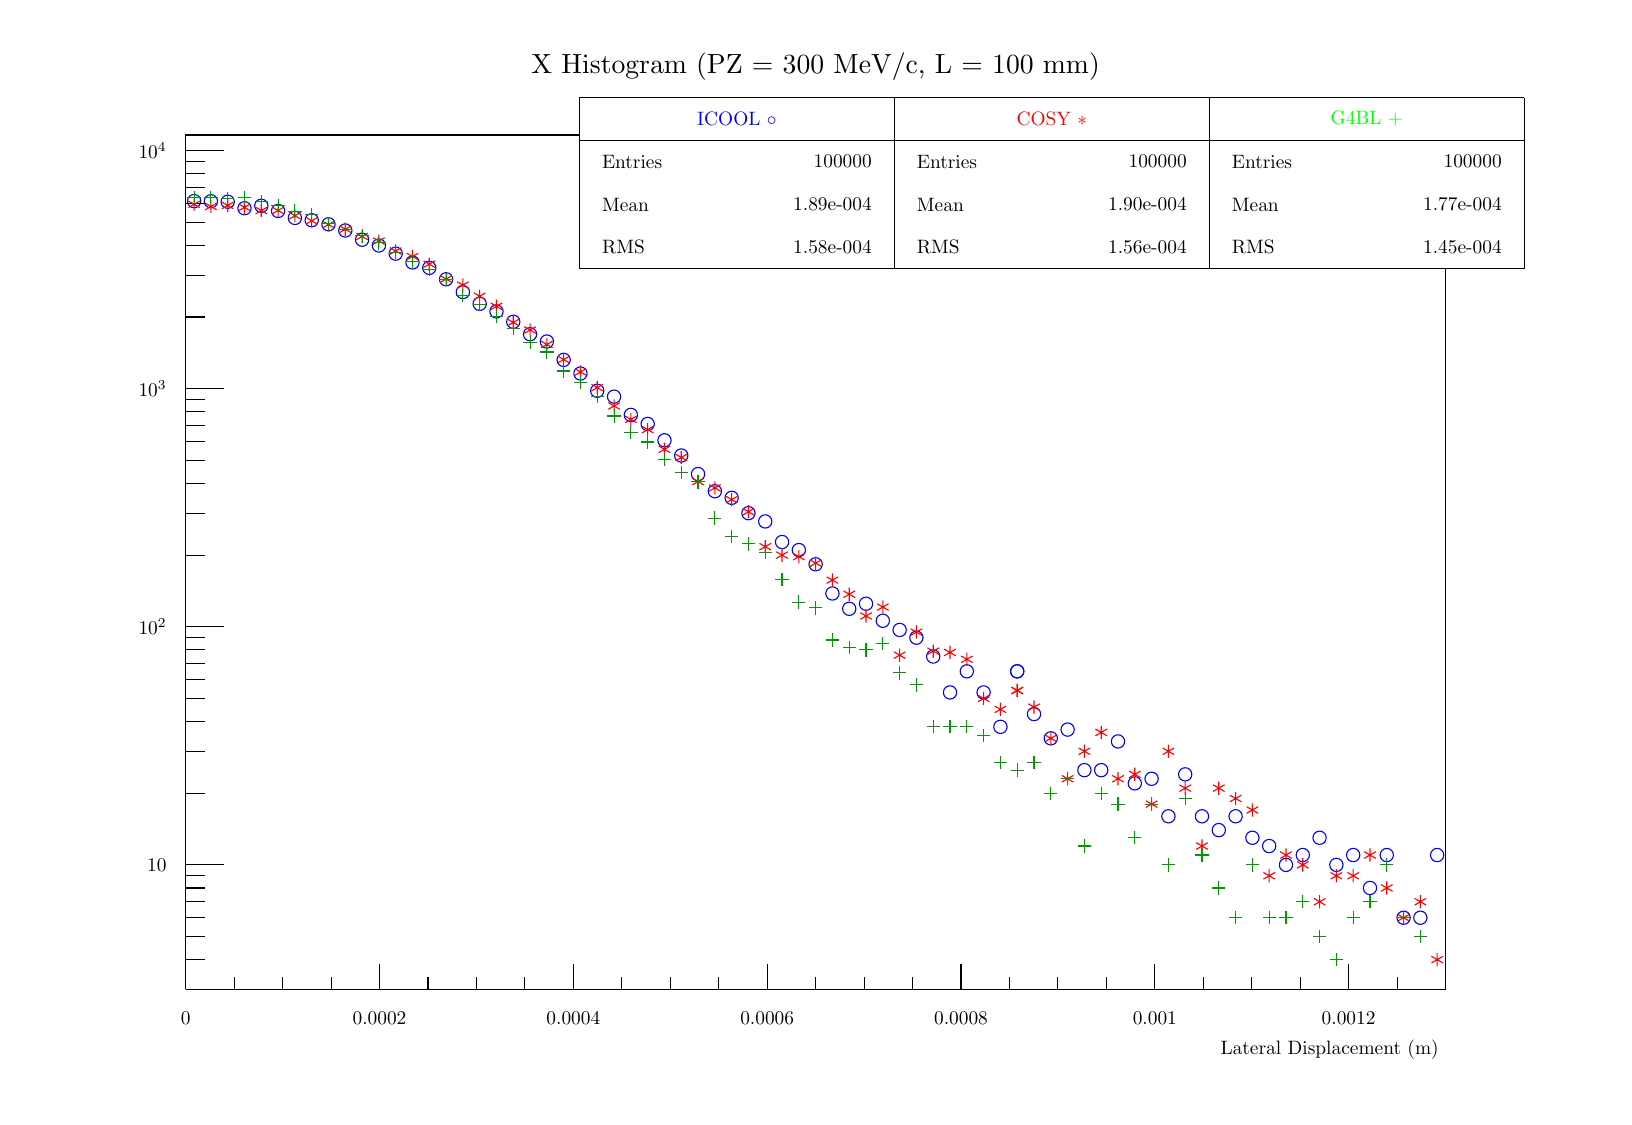
\begin{tikzpicture}
\definecolor{c}{rgb}{1,1,1};
\draw [color=c, fill=c] (0,0) rectangle (20,13.5632);
\draw [color=c, fill=c] (2,1.35632) rectangle (18,12.2069);
\definecolor{c}{rgb}{0,0,0};
\draw [c] (2,1.35632) -- (2,12.2069) -- (18,12.2069) -- (18,1.35632) -- (2,1.35632);
\definecolor{c}{rgb}{1,1,1};
\draw [color=c, fill=c] (2,1.35632) rectangle (18,12.2069);
\definecolor{c}{rgb}{0,0,0};
\draw [c] (2,1.35632) -- (2,12.2069) -- (18,12.2069) -- (18,1.35632) -- (2,1.35632);
\definecolor{c}{rgb}{0,0,1};
\foreach \P in
 {(2.10667,11.3676),(2.32,11.3655),(2.53333,11.3592),(2.74667,11.2763),(2.96,11.3081),(3.17333,11.2426),(3.38667,11.154),(3.6,11.1247),(3.81333,11.073),(4.02667,10.9943),(4.24,10.8775),(4.45333,10.8039),(4.66667,10.7003),(4.88,10.5882),(5.09333,10.51
98),(5.30667,10.3745),(5.52,10.2126),(5.73333,10.0625),(5.94667,9.96655),(6.16,9.83514),(6.37333,9.67676),(6.58667,9.58438),(6.8,9.35092),(7.01333,9.17797),(7.22667,8.95879),(7.44,8.88435),(7.65333,8.65227),(7.86667,8.53738),(8.08,8.3297),(8.29333,8.
1366),(8.50667,7.90116),(8.72,7.68314),(8.93333,7.59909),(9.14667,7.40417),(9.36,7.29942),(9.57333,7.03799),(9.78667,6.93576),(10,6.75502),(10.2133,6.38438),(10.4267,6.18984),(10.64,6.25444),(10.8533,6.03792),(11.0667,5.92139),(11.28,5.82303),(11.493
3,5.58359),(11.7067,5.12762),(11.92,5.39566),(12.1333,5.12762),(12.3467,4.69069),(12.56,5.39566)}{\draw[mark options={color=c,fill=c},mark size=2.402402pt,mark=o] plot coordinates {\P};}
\foreach \P in
 {(12.56,5.39566),(12.7733,4.85303),(12.9867,4.54462),(13.2,4.65567),(13.4133,4.14081),(13.6267,4.14081),(13.84,4.50541),(14.0533,3.97293),(14.2667,4.03131),(14.48,3.55471),(14.6933,4.0872),(14.9067,3.55471),(15.12,3.37935),(15.3333,3.55471),(15.5467
,3.28202),(15.76,3.17691),(15.9733,2.93747),(16.1867,3.06264),(16.4,3.28202),(16.6133,2.93747),(16.8267,3.06264),(17.04,2.64442),(17.2533,3.06264),(17.4667,2.26661),(17.68,2.26661),(17.8933,3.06264)}{\draw[mark options={color=c,fill=c},mark
 size=2.402402pt,mark=o] plot coordinates {\P};}
\definecolor{c}{rgb}{1,1,1};
\draw [color=c, fill=c] (7,10.5115) rectangle (11,12.6816);
\definecolor{c}{rgb}{0,0,0};
\draw [c] (7,10.5115) -- (11,10.5115);
\draw [c] (11,10.5115) -- (11,12.6816);
\draw [c] (11,12.6816) -- (7,12.6816);
\draw [c] (7,12.6816) -- (7,10.5115);
\draw[color=blue](9,12.4103) node[scale=0.7, rotate=0]{ICOOL $\circ$};
\draw [c] (7,12.1391) -- (11,12.1391);
\draw [anchor= west] (7.2,11.8678) node[scale=0.7, rotate=0]{Entries };
\draw [anchor= east] (10.8,11.8678) node[scale=0.7, rotate=0]{ 100000};
\draw [anchor= west] (7.2,11.3253) node[scale=0.7, rotate=0]{Mean  };
\draw [anchor= east] (10.8,11.3253) node[scale=0.7, rotate=0]{ 1.89e-004};
\draw [anchor= west] (7.2,10.7828) node[scale=0.7, rotate=0]{RMS   };
\draw [anchor= east] (10.8,10.7828) node[scale=0.7, rotate=0]{ 1.58e-004};
\draw [c] (2,1.35632) -- (18,1.35632);
\draw [anchor= east] (18,0.596782) node[scale=0.7, rotate=0]{Lateral Displacement (m)};
\draw [c] (2,1.68184) -- (2,1.35632);
\draw [c] (2.61538,1.51908) -- (2.61538,1.35632);
\draw [c] (3.23077,1.51908) -- (3.23077,1.35632);
\draw [c] (3.84615,1.51908) -- (3.84615,1.35632);
\draw [c] (4.46154,1.68184) -- (4.46154,1.35632);
\draw [c] (5.07692,1.51908) -- (5.07692,1.35632);
\draw [c] (5.69231,1.51908) -- (5.69231,1.35632);
\draw [c] (6.30769,1.51908) -- (6.30769,1.35632);
\draw [c] (6.92308,1.68184) -- (6.92308,1.35632);
\draw [c] (7.53846,1.51908) -- (7.53846,1.35632);
\draw [c] (8.15385,1.51908) -- (8.15385,1.35632);
\draw [c] (8.76923,1.51908) -- (8.76923,1.35632);
\draw [c] (9.38461,1.68184) -- (9.38461,1.35632);
\draw [c] (10,1.51908) -- (10,1.35632);
\draw [c] (10.6154,1.51908) -- (10.6154,1.35632);
\draw [c] (11.2308,1.51908) -- (11.2308,1.35632);
\draw [c] (11.8462,1.68184) -- (11.8462,1.35632);
\draw [c] (12.4615,1.51908) -- (12.4615,1.35632);
\draw [c] (13.0769,1.51908) -- (13.0769,1.35632);
\draw [c] (13.6923,1.51908) -- (13.6923,1.35632);
\draw [c] (14.3077,1.68184) -- (14.3077,1.35632);
\draw [c] (14.9231,1.51908) -- (14.9231,1.35632);
\draw [c] (15.5385,1.51908) -- (15.5385,1.35632);
\draw [c] (16.1538,1.51908) -- (16.1538,1.35632);
\draw [c] (16.7692,1.68184) -- (16.7692,1.35632);
\draw [c] (16.7692,1.68184) -- (16.7692,1.35632);
\draw [c] (17.3846,1.51908) -- (17.3846,1.35632);
\draw [c] (18,1.51908) -- (18,1.35632);
\draw [anchor=base] (2,0.908736) node[scale=0.7, rotate=0]{0};
\draw [anchor=base] (4.46154,0.908736) node[scale=0.7, rotate=0]{0.0002};
\draw [anchor=base] (6.92308,0.908736) node[scale=0.7, rotate=0]{0.0004};
\draw [anchor=base] (9.38461,0.908736) node[scale=0.7, rotate=0]{0.0006};
\draw [anchor=base] (11.8462,0.908736) node[scale=0.7, rotate=0]{0.0008};
\draw [anchor=base] (14.3077,0.908736) node[scale=0.7, rotate=0]{0.001};
\draw [anchor=base] (16.7692,0.908736) node[scale=0.7, rotate=0]{0.0012};
\draw [c] (2,1.35632) -- (2,12.2069);
\draw [c] (2.24,1.73412) -- (2,1.73412);
\draw [c] (2.24,2.02717) -- (2,2.02717);
\draw [c] (2.24,2.26661) -- (2,2.26661);
\draw [c] (2.24,2.46905) -- (2,2.46905);
\draw [c] (2.24,2.64442) -- (2,2.64442);
\draw [c] (2.24,2.7991) -- (2,2.7991);
\draw [c] (2.48,2.93747) -- (2,2.93747);
\draw [anchor= east] (1.844,2.93747) node[scale=0.7, rotate=0]{10};
\draw [c] (2.24,3.84776) -- (2,3.84776);
\draw [c] (2.24,4.38024) -- (2,4.38024);
\draw [c] (2.24,4.75805) -- (2,4.75805);
\draw [c] (2.24,5.0511) -- (2,5.0511);
\draw [c] (2.24,5.29054) -- (2,5.29054);
\draw [c] (2.24,5.49298) -- (2,5.49298);
\draw [c] (2.24,5.66834) -- (2,5.66834);
\draw [c] (2.24,5.82302) -- (2,5.82302);
\draw [c] (2.48,5.96139) -- (2,5.96139);
\draw [anchor= east] (1.844,5.96139) node[scale=0.7, rotate=0]{$10^{2}$};
\draw [c] (2.24,6.87168) -- (2,6.87168);
\draw [c] (2.24,7.40417) -- (2,7.40417);
\draw [c] (2.24,7.78198) -- (2,7.78198);
\draw [c] (2.24,8.07502) -- (2,8.07502);
\draw [c] (2.24,8.31446) -- (2,8.31446);
\draw [c] (2.24,8.5169) -- (2,8.5169);
\draw [c] (2.24,8.69227) -- (2,8.69227);
\draw [c] (2.24,8.84695) -- (2,8.84695);
\draw [c] (2.48,8.98532) -- (2,8.98532);
\draw [anchor= east] (1.844,8.98532) node[scale=0.7, rotate=0]{$10^{3}$};
\draw [c] (2.24,9.89561) -- (2,9.89561);
\draw [c] (2.24,10.4281) -- (2,10.4281);
\draw [c] (2.24,10.8059) -- (2,10.8059);
\draw [c] (2.24,11.0989) -- (2,11.0989);
\draw [c] (2.24,11.3384) -- (2,11.3384);
\draw [c] (2.24,11.5408) -- (2,11.5408);
\draw [c] (2.24,11.7162) -- (2,11.7162);
\draw [c] (2.24,11.8709) -- (2,11.8709);
\draw [c] (2.48,12.0092) -- (2,12.0092);
\draw [anchor= east] (1.844,12.0092) node[scale=0.7, rotate=0]{$10^{4}$};
\definecolor{c}{rgb}{1,1,1};
\draw [color=c, fill=c] (7,10.5115) rectangle (11,12.6816);
\definecolor{c}{rgb}{0,0,0};
\draw [c] (7,10.5115) -- (11,10.5115);
\draw [c] (11,10.5115) -- (11,12.6816);
\draw [c] (11,12.6816) -- (7,12.6816);
\draw [c] (7,12.6816) -- (7,10.5115);
\draw[color=blue](9,12.4103) node[scale=0.7, rotate=0]{ICOOL $\circ$};
\draw [c] (7,12.1391) -- (11,12.1391);
\draw [anchor= west] (7.2,11.8678) node[scale=0.7, rotate=0]{Entries };
\draw [anchor= east] (10.8,11.8678) node[scale=0.7, rotate=0]{ 100000};
\draw [anchor= west] (7.2,11.3253) node[scale=0.7, rotate=0]{Mean  };
\draw [anchor= east] (10.8,11.3253) node[scale=0.7, rotate=0]{ 1.89e-004};
\draw [anchor= west] (7.2,10.7828) node[scale=0.7, rotate=0]{RMS   };
\draw [anchor= east] (10.8,10.7828) node[scale=0.7, rotate=0]{ 1.58e-004};
\draw (10,13.0816) node[scale=1, rotate=0]{X Histogram (PZ = 300 MeV/c, L = 100 mm)};
\definecolor{c}{rgb}{1,0,0};
\foreach \P in
 {(2.10667,11.3267),(2.32,11.2991),(2.53333,11.3127),(2.74667,11.2882),(2.96,11.2473),(3.17333,11.2485),(3.38667,11.1817),(3.6,11.1172),(3.81333,11.0692),(4.02667,11.0096),(4.24,10.9188),(4.45333,10.8606),(4.66667,10.734),(4.88,10.6635),(5.09333,10.5
667),(5.30667,10.3772),(5.52,10.3009),(5.73333,10.1594),(5.94667,10.0315),(6.16,9.82548),(6.37333,9.72997),(6.58667,9.54638),(6.8,9.35489),(7.01333,9.19711),(7.22667,8.99838),(7.44,8.76569),(7.65333,8.5952),(7.86667,8.46525),(8.08,8.21444),(8.29333,8
.11129),(8.50667,7.80476),(8.72,7.72494),(8.93333,7.57625),(9.14667,7.42157),(9.36,6.97882),(9.57333,6.87168),(9.78667,6.85184),(10,6.7693),(10.2133,6.55378),(10.4267,6.37483),(10.64,6.09845),(10.8533,6.21173),(11.0667,5.60098),(11.28,5.89403),(11.49
33,5.65182),(11.7067,5.63509),(11.92,5.54809),(12.1333,5.0511),(12.3467,4.91273),(12.56,5.15217)}{\draw[mark options={color=c,fill=c},mark size=2.402402pt,mark=asterisk] plot coordinates {\P};}
\foreach \P in
 {(12.56,5.15217),(12.7733,4.9416),(12.9867,4.54462),(13.2,4.03131),(13.4133,4.38025),(13.6267,4.61968),(13.84,4.03131),(14.0533,4.0872),(14.2667,3.70939),(14.48,4.38025),(14.6933,3.91183),(14.9067,3.17691),(15.12,3.91183),(15.3333,3.7804),(15.5467,3
.63433),(15.76,2.7991),(15.9733,3.06264),(16.1867,2.93747),(16.4,2.46906),(16.6133,2.7991),(16.8267,2.7991),(17.04,3.06264),(17.2533,2.64442),(17.4667,2.26661),(17.68,2.46906),(17.8933,1.73413)}{\draw[mark options={color=c,fill=c},mark
 size=2.402402pt,mark=asterisk] plot coordinates {\P};}
\definecolor{c}{rgb}{1,1,1};
\draw [color=c, fill=c] (11,10.5115) rectangle (15,12.6816);
\definecolor{c}{rgb}{0,0,0};
\draw [c] (11,10.5115) -- (15,10.5115);
\draw [c] (15,10.5115) -- (15,12.6816);
\draw [c] (15,12.6816) -- (11,12.6816);
\draw [c] (11,12.6816) -- (11,10.5115);
\draw [color=red](13,12.4103) node[scale=0.7, rotate=0]{COSY $*$};
\draw [c] (11,12.1391) -- (15,12.1391);
\draw [anchor= west] (11.2,11.8678) node[scale=0.7, rotate=0]{Entries };
\draw [anchor= east] (14.8,11.8678) node[scale=0.7, rotate=0]{ 100000};
\draw [anchor= west] (11.2,11.3253) node[scale=0.7, rotate=0]{Mean  };
\draw [anchor= east] (14.8,11.3253) node[scale=0.7, rotate=0]{ 1.90e-004};
\draw [anchor= west] (11.2,10.7828) node[scale=0.7, rotate=0]{RMS   };
\draw [anchor= east] (14.8,10.7828) node[scale=0.7, rotate=0]{ 1.56e-004};
\definecolor{c}{rgb}{1,1,1};
\draw [color=c, fill=c] (11,10.5115) rectangle (15,12.6816);
\definecolor{c}{rgb}{0,0,0};
\draw [c] (11,10.5115) -- (15,10.5115);
\draw [c] (15,10.5115) -- (15,12.6816);
\draw [c] (15,12.6816) -- (11,12.6816);
\draw [c] (11,12.6816) -- (11,10.5115);
\draw [color=red](13,12.4103) node[scale=0.7, rotate=0]{COSY $*$};
\draw [c] (11,12.1391) -- (15,12.1391);
\draw [anchor= west] (11.2,11.8678) node[scale=0.7, rotate=0]{Entries };
\draw [anchor= east] (14.8,11.8678) node[scale=0.7, rotate=0]{ 100000};
\draw [anchor= west] (11.2,11.3253) node[scale=0.7, rotate=0]{Mean  };
\draw [anchor= east] (14.8,11.3253) node[scale=0.7, rotate=0]{ 1.90e-004};
\draw [anchor= west] (11.2,10.7828) node[scale=0.7, rotate=0]{RMS   };
\draw [anchor= east] (14.8,10.7828) node[scale=0.7, rotate=0]{ 1.56e-004};
\definecolor{c}{rgb}{0,0.6,0};
\foreach \P in
 {(2.10667,11.4102),(2.32,11.417),(2.53333,11.3983),(2.74667,11.4133),(2.96,11.3577),(3.17333,11.3076),(3.38667,11.241),(3.6,11.1939),(3.81333,11.0823),(4.02667,11.0051),(4.24,10.9251),(4.45333,10.837),(4.66667,10.7152),(4.88,10.6006),(5.09333,10.504
2),(5.30667,10.3676),(5.52,10.1659),(5.73333,10.0515),(5.94667,9.9002),(6.16,9.75212),(6.37333,9.57015),(6.58667,9.45136),(6.8,9.21045),(7.01333,9.05936),(7.22667,8.88435),(7.44,8.63866),(7.65333,8.42964),(7.86667,8.30788),(8.08,8.08549),(8.29333,7.9
2493),(8.50667,7.80153),(8.72,7.34141),(8.93333,7.11112),(9.14667,7.01464),(9.36,6.90411),(9.57333,6.56212),(9.78667,6.27529),(10,6.20083),(10.2133,5.79351),(10.4267,5.70077),(10.64,5.66834),(10.8533,5.74796),(11.0667,5.3753),(11.28,5.22318),(11.4933
,4.69069),(11.7067,4.69069),(11.92,4.69069),(12.1333,4.58269),(12.3467,4.24188),(12.56,4.14081)}{\draw[mark options={color=c,fill=c},mark size=2.402402pt,mark=+] plot coordinates {\P};}
\foreach \P in
 {(12.56,4.14081),(12.7733,4.24188),(12.9867,3.84776),(13.2,4.03131),(13.4133,3.17691),(13.6267,3.84776),(13.84,3.70939),(14.0533,3.28202),(14.2667,3.70939),(14.48,2.93747),(14.6933,3.7804),(14.9067,3.06264),(15.12,2.64442),(15.3333,2.26661),(15.5467
,2.93747),(15.76,2.26661),(15.9733,2.26661),(16.1867,2.46906),(16.4,2.02718),(16.6133,1.73413),(16.8267,2.26661),(17.04,2.46906),(17.2533,2.93747),(17.4667,2.26661),(17.68,2.02718)}{\draw[mark options={color=c,fill=c},mark size=2.402402pt,mark=+]
 plot coordinates {\P};}
\definecolor{c}{rgb}{1,1,1};
\draw [color=c, fill=c] (15,10.5115) rectangle (19,12.6816);
\definecolor{c}{rgb}{0,0,0};
\draw [c] (15,10.5115) -- (19,10.5115);
\draw [c] (19,10.5115) -- (19,12.6816);
\draw [c] (19,12.6816) -- (15,12.6816);
\draw [c] (15,12.6816) -- (15,10.5115);
\draw [color=green](17,12.4103) node[scale=0.7, rotate=0]{G4BL $+$};
\draw [c] (15,12.1391) -- (19,12.1391);
\draw [anchor= west] (15.2,11.8678) node[scale=0.7, rotate=0]{Entries };
\draw [anchor= east] (18.8,11.8678) node[scale=0.7, rotate=0]{ 100000};
\draw [anchor= west] (15.2,11.3253) node[scale=0.7, rotate=0]{Mean  };
\draw [anchor= east] (18.8,11.3253) node[scale=0.7, rotate=0]{ 1.77e-004};
\draw [anchor= west] (15.2,10.7828) node[scale=0.7, rotate=0]{RMS   };
\draw [anchor= east] (18.8,10.7828) node[scale=0.7, rotate=0]{ 1.45e-004};
\definecolor{c}{rgb}{1,1,1};
\draw [color=c, fill=c] (15,10.5115) rectangle (19,12.6816);
\definecolor{c}{rgb}{0,0,0};
\draw [c] (15,10.5115) -- (19,10.5115);
\draw [c] (19,10.5115) -- (19,12.6816);
\draw [c] (19,12.6816) -- (15,12.6816);
\draw [c] (15,12.6816) -- (15,10.5115);
\draw [color=green](17,12.4103) node[scale=0.7, rotate=0]{G4BL $+$};
\draw [c] (15,12.1391) -- (19,12.1391);
\draw [anchor= west] (15.2,11.8678) node[scale=0.7, rotate=0]{Entries };
\draw [anchor= east] (18.8,11.8678) node[scale=0.7, rotate=0]{ 100000};
\draw [anchor= west] (15.2,11.3253) node[scale=0.7, rotate=0]{Mean  };
\draw [anchor= east] (18.8,11.3253) node[scale=0.7, rotate=0]{ 1.77e-004};
\draw [anchor= west] (15.2,10.7828) node[scale=0.7, rotate=0]{RMS   };
\draw [anchor= east] (18.8,10.7828) node[scale=0.7, rotate=0]{ 1.45e-004};
\end{tikzpicture}
